\documentclass[11pt]{article}

\usepackage{epsfig}
\usepackage{amsfonts}
\usepackage{amssymb}
\usepackage{amstext}
\usepackage{amsmath}
\usepackage{xspace}
\usepackage{theorem}
\usepackage{hyperref}
\usepackage{fullpage}
\usepackage{enumitem}
\usepackage{graphicx}
\usepackage{indentfirst}
\usepackage[dvipsnames]{xcolor}
\usepackage{xeCJK}
\setCJKmainfont{IPAMincho}
\setCJKsansfont{IPAGothic}
\setCJKmonofont{IPAGothic}

\usepackage{listings}

\usepackage{enumitem}                     


\usepackage{titlesec}

\titleformat*{\section}{\bfseries}
\titleformat*{\subsection}{\bfseries}
\titleformat*{\subsubsection}{\bfseries}
\titleformat*{\paragraph}{\bfseries}
\titleformat*{\subparagraph}{\bfseries}


\newenvironment{proof}{{\bf Proof:  }}{\hfill\rule{2mm}{2mm}}
\newenvironment{proofof}[1]{{\bf Proof of #1:  }}{\hfill\rule{2mm}{2mm}}
\newenvironment{proofofnobox}[1]{{\bf#1:  }}{}
\newenvironment{example}{{\bf Example:  }}{\hfill\rule{2mm}{2mm}}


\newtheorem{fact}{Fact}[section]
\newtheorem{lemma}[fact]{Lemma}
\newtheorem{theorem}[fact]{Theorem}
\newtheorem{definition}[fact]{Definition}
\newtheorem{corollary}[fact]{Corollary}
\newtheorem{proposition}[fact]{Proposition}
\newtheorem{claim}[fact]{Claim}
\newtheorem{exercise}[fact]{Exercise}

% math notation
\newcommand{\R}{\ensuremath{\mathbb R}}
\newcommand{\Z}{\ensuremath{\mathbb Z}}
\newcommand{\N}{\ensuremath{\mathbb N}}
\newcommand{\F}{\ensuremath{\mathcal F}}
\newcommand{\SymGrp}{\ensuremath{\mathfrak S}}

\newcommand{\size}[1]{\ensuremath{\left|#1\right|}}
\newcommand{\ceil}[1]{\ensuremath{\left\lceil#1\right\rceil}}
\newcommand{\floor}[1]{\ensuremath{\left\lfloor#1\right\rfloor}}
\newcommand{\poly}{\operatorname{poly}}
\newcommand{\polylog}{\operatorname{polylog}}

% anupam's abbreviations
\newcommand{\e}{\epsilon}
\newcommand{\half}{\ensuremath{\frac{1}{2}}}
\newcommand{\junk}[1]{}
\newcommand{\sse}{\subseteq}
\newcommand{\union}{\cup}
\newcommand{\meet}{\wedge}

\newcommand{\prob}[1]{\ensuremath{\text{{\bf Pr}$\left[#1\right]$}}}
\newcommand{\expct}[1]{\ensuremath{\text{{\bf E}$\left[#1\right]$}}}
\newcommand{\Event}{{\mathcal E}}

\newcommand{\mnote}[1]{\normalmarginpar \marginpar{\tiny #1}}

\setenumerate[0]{label=(\alph*)}
\setcounter{tocdepth}{4}
\setcounter{secnumdepth}{4}

\usepackage[
backend=biber,
style=alphabetic,
]{biblatex}
\addbibresource{citations.bib}

%%%%%%%%%%%%%%%%%%%%%%%%%%%%%%%%%%%%%%%%%%%%%%%%%%%%%%%%%%%%%%%%%%%%%%%%%%%
% Document begins here %%%%%%%%%%%%%%%%%%%%%%%%%%%%%%%%%%%%%%%%%%%%%%%%%%%%
%%%%%%%%%%%%%%%%%%%%%%%%%%%%%%%%%%%%%%%%%%%%%%%%%%%%%%%%%%%%%%%%%%%%%%%%%%%



\begin{document}
\title{Multi Politeness-Domain Neural Machine Translation for Japanese and Korean}

\author{Henry Li Xinyuan, Jerry Chen, Ray Lee}

\date{Autumn 2021}

\maketitle

\newpage

\section{Introduction}

\subsection{Motivation}

Language can work in extremely subtle ways, and sometimes very small changes can drastically alter the undertone of a sentence or an utterance \cite{Feely:19} \cite{niu-etal-2018-multi}: tiny details such as intonation, conjugation, choice of vocabulary, as well as many factors that would often be overlooked by neural models when extracting meaning \cite{pavlick-tetreault-2016-empirical}. While general sequence-to-sequence machine translation is capable of producing results that are very coherent and semantically close to the target output, small details such as formality can often be neglected by the model \cite{rao2018dear} - details that can make or break a career if approached carelessly by a human. As such, we propose systems that aim at adapting existing neural machine translation architectures, so that they would be able to classify sentences according to their formality and reproduce sentences in the correct formality class. 

\subsection{Problem Description}

Formality is almost universal across all languages \cite{article}, and yet there are certain languages that have more clearly identifiable formality markers. Some of these languages are Japanese and Korean, both of which exhibit different verb conjugations for different formality classes. Identifying sentence formality in other languages without such clear markers, such as English, is a non-trivial problem \cite{pavlick-tetreault-2016-empirical} and is beyond the scope of our study. 

In short, we would like our model to be able to perform two additional tasks, on top of translation:

\begin{enumerate}[label=\arabic*]
    \item Indentify the formality class of the input sentence;
    \item Emit sentences in the target language with the correct formality class (which is either given as input, or generated automatically according to the input sentence).
\end{enumerate}

More generally, we want to build NMT models that can correctly infer morphologies, inflections, as well as choose the correct word among a set of words that are semantically close, or which the problem introduced in this study can be seen as a special case.

\section{Training Data}

\subsection{Choice of Corpus}

Countless corpora of Japanese exist on the Internet, yet the ones that would be suitable for our needs are far and few between. There is typically a strong correlation between formality and context, which is not bad news for us since relying purely on morphology to label formality would have problems of its own. However, we want to avoid introducing into our corpus large chunks of sentences with the same context in the same formality domain, lest any of our models learns to classify contexts rather than formality. Many such examples of bad corpora exist, such as the corpus of Japanese legal documents: in Japanese, all legal documents are written in informal form (contrary to what one might assume); we must be very careful when using such corpora by balancing and mixing them with corpora from other sources and with different formality domains. Examples of good corpora include the subtitle corpus, although the translation quality of some of the sentences in that corpus has been questioned. In general, Japanese is a more context-based language, and it often leaves out parts of the phrase than can be inferred. In most cases, this means omitting the subject. This means that English translation will generally have more context than the Japanese equivalent. Currently, there are no corpora that avoid this issue, as any such corpus would have to be either laboriously picked out or have a heavy bias toward formal sentences. As such, it may be that Japanese to English translation ``predicts" a subject, as one is required in English. 

\subsection{Politeness Labels}

We designed our model to be able to handle both translation and formality classification. While extracting a representation for politeness from the automatically extracted features in a neural network pipeline isn't impossible, that is not what we are trying to achieve. Rather, we would train our model under a supervised learning scheme, where each sentence has a corresponding ground truth translation and formality label attached.

One of the earliest roadblocks we faced is the scarcity of such sentence-formality pairs. Such corpora are extremely difficult to find in sufficient quantities that would allow for adequate training of a neural classification model. Human annotation is unfortunately not so accessible for Japanese (in terms of pricing) as some other languages. As such, we devised a number of ways to generated such sentence-formality pairs.

\subsubsection{Procedural Generation of Politeness Labels}

Fortunately for us, this is a topic that had been studied previously by Feely et al. \cite{Feely:19}, which in turn was based on the Kyoto Text Analysis Toolkit (KyTea) \cite{Neubig:11}. In their case, Japanese was the destination language; the task was to generate Japanese sentences that would match the formality levels of the input. 

The authors identified verb suffixes and copulas as the keys for indentifying sentence formality, with short-form corresponding to informal sentences and long-form corresponding to formal ones. They published a conversion script which would identify and convert any informal verb suffixes into formal verb suffixes, and vice versa. There is a slight complication to this rule, which is that in Japanese there are situations which constrain the verb to be short-form, ie. when it forms part of a verb phrase that isn't the head of the sentence. Fortunately, Japanese is also a language which observes the SOV order, meaning that the final verb in a sentence is always the head verb and is never constrained to short form. As such, we can first perform sentence tokenisation and then use the long-short form of the final verb/copula in each sentence to determine its formality. There are some exceptions to this SOV structure, especially in the short-form, and especially involving the omission of the verb ``desu", (translated as ``to be"). Fortunately, in these cases, the final term is an adjective, which in Japanese also conjugate in a way that's distinguishable by politeness. 

We thus from their script and make two important modifications. First we adapt their conversion script into a classification script. We also take advantage of the fact that the formality level in a single document should remain the same. This observation can serve multiple purposes:

\begin{enumerate}[label=\arabic*]
    \item A sanity check for the outputs of our script;
    \item Simplify our calculation for classifying sentences that had been segmented into documents.
\end{enumerate}

We performed a sanity check on the legal corpus we mentioned earlier (a corpus entirely made up of informal sentences) and got very positive results: not a single sentence in the corpus of $262000$ lines were identified as formal.

Some corpora are already tokenised at sentence level and do not form part of a document, and we were forced to weaken our common-formality assumption to individual corpus entries (which may contain multiple sentences). 

One problem that we faced with Japanese-English translation was that Japanese is a language with strong formality and honorifics and English is a language with very weak formality. Thus, we sought to find something similar to Feely et al.'s work, but in Korean. Bravender's open-source application on conjugating Korean verbs proved useful to us.

Bravender's application, koreanverb.app, takes in a Korean verb as an input, and outputs the stem and different conjugations, taking into account tense, formality, and types of statements, such as declarative, imperative, and so on. We believed that this tool would be useful in determining whether the Korean sentences in the corpora we choose to use are formal or informal.

Since Korean is a language that observes SOV order like Japanese, we followed similar steps as we had done previously for analyzing the formality of a given Korean sentence. After tokenizing Korean sentences, we would detect the last verb in the sentence. Then, by using methods from Bravender's application, we would analyze the verb to see whether it was in a formal (or high, in Bravender's code) form or an informal (or low) form.

The procedural classification scripts put each sentence into one of $3$ bins (formal, informal, inconclusive) according to the above-mentioned rules. Note the presence of the "inconclusive" class: these are the sentences that don't contain a formality marker (such as a well-conjugated verb, a copula, or an adjective): in some corpora (such as the subtitles corpus) they account for around one-third of the sentences. We simplify the task for our model by removing all inconclusive sentences and making formality classification a binary-classification task. 

Due to the nature of the corpora that we chose, informal sentences outnumber formal sentences. We therefore randomly drop some informal sentences so that the number of formal and informal sentences are roughly equal.

\subsubsection{Using Pre-trained Japanese Language Model for Politeness Labelling}

While Japanese is not nearly as high-resource as English (GPT-3 was never specifically trained on Japanese, for example), there are nevertheless some available pre-trained Japanese language models that are available. One of the best recent models that were developed is the Japanese BERT trained at Tohoku University. Similar to the original BERT, this model performs a mask-filling task on Japanese sentences. 

The obvious way of making use of a pre-trained language model for politeness labelling would be to fine-tuned it on the new task. However, that would require correctly labelled data, leading us to a chicken-and-egg problem. Alternatively we could use the labels that we generated in section $1.2.1$, although then we would be constrained by the quality of our previous scoring function.

A slightly modified approach would be: for each sentence, we identify and mask each verb (along with its suffix conjugation) and each copula one at a time. We feed the masked sentences to the language model. We then score each sentence based on whether the language model filled the masks with long forms or short forms.

\paragraph{BERT Fine-tuned on Formality Classification}

The setup for this experiment is simple: we take a pre-trained Japanese language model and attempt to fine tune it with the sentence-formality label pairs that we generated in section $1.2.1$. We first try viewing this problem as a scoring problem, with the model tuned to produce a score between $0$ and $1$ for each document and with a score greater than $.5$ indicating that the model considers the document to be formal, and vice versa. We tried two different experimental settings, one where ambiguous sentences (those that didn't contain a formality indicator) are mixed in with target score $.5$, the other where ambiguous sentences are not included.

The other approach is to regard the problem as a two-class classification task. We do not introduce a third class of ambiguous sentences under this setting, since it is questionable from a linguistic point of view to label these sentences as "formality-free". This is the approach which we experimented on.

The pre-trained model that we used was BertJapanese, developed by Masatoshi Suzuki at the Tohoku NLP lab and available in the transformers package by huggingface. The model converts a character-tokenised sentence into a $768$-dimension embedding which we use as the output for our classifier. Given the low dimensionality of our output, we choose the simplest model architecture possible: a one-layer perceptron with a non-linearity (sigmoid), a linear layer and a log softmax output processing layer.

In our experiments, we were able to achieve a labelling accuracy of $.794$ for our generated formality label data. We observe similar movements in train and dev accuracy and loss during training, as well as comparable test accuracy compared to train and dev accuracy. Given the size of our test data set ($152576$), we believe our results are robust and not the result of any fortuitous statistical event.

We compare those results to the ones we achieved from a BERT model based on word tokenisation. The accuracy was comparable to the character-based BERT, at $.787$, however there was a substantial runtime reduction due to word-level tokenised sequences being shorter than character-level tokenised ones (average length of a Japanese word is around $2$ characters, however we would expect - and did observe - speedup less than $50\%$ due to punctuations, numbers, non-Japanese characters, etc.). 

\paragraph{Masking Decisive Verb/Copula}

This setup doesn't even require any fine-tuning, simply deploying existing mask-fill language models and masking the correct words would suffice. We did not build such a system since the baseline was satisfactory and this is not the focus of our study. For more information, please refer to an earlier study of posterior manipulation of black box language models by Li and Rush \cite{DBLP:journals/corr/abs-2005-04560}.

\subsubsection{Other Techniques for Politeness Labelling}

Some other techniques for politeness labelling of Japanese and other languages had been proposed, and we will discuss them briefly here. Dugan \cite{Dugan:20} proposed generating politeness labels from the corresponding English translation, an idea we didn't find convincing due to the inherent problems associated with inferring formality from English which has relatively few clear markers for formality, not the mention the problem with noise introduced by otherwise perfect translations with incorrect formality.

\section{Model Architecture}

A number of possible architectures could be used to integrate the translation task with the formality labelling task. We implement a number of thems, comparing their performance when their tasks are comparable.

\subsection{Base translation model without formality labels}

We first build a base translation model that doesn't take formality into account. We will use its performance as a baseline and attempt to beat its performance with our formality-aware model. For test cases where either the source or the target language doesn't have strong formality classes (such as Japanese-English or vice versa), we are only interested in the translation quality. For cases where both the source and the target language have strong formality classes (such as Korean-Japanese), we are also interested in formality class correspondance.

The base translation model we choose for our task an autoregressive transformer model \cite{vaswani2017attention}, which was selected due to its success in machine translation \cite{liu2020deep}. The encoder-decoder construction is significant for us, since the pooled encoder output is going to be the basis for our formality classifier (similar to what we did with the pre-trained Japanese BERT).

Due to the autoregressive nature of our model, in the interest of time saving, we limit the maximum length of each sentence to $15$. Sentences that had a greater length were discarded.

For Japanese language pre-processing, we relied on the sentence tokenisation tool by Mecab \cite{Kudo2005MeCabY}. For pre-processing English sentences, we used the tokenisation tool by fairseq \cite{ott2019fairseq}.

We encountered significant difficulties when constructing the base Japanese to English translator. Due to the diverse and noisy nature of our corpus, as well as the tendency towards subject omission in Japanese, our translator could not perform even the most basic translation task, regardless of the hyper-parameters we choose. We found that careful pre-processing of our data goes a long way to helping the performance of the base translator: after pruning our dataset down to around $20\%$ its original size and consisting only of grammatically complete sentences, our model could reach a respectable performance on the held-out part of the cleaned dataset ($26.3$ BLEU score) while also perform reasonably well on the original larger dataset.

\subsection{Base Autoencoder-Reconstructor}

This can be seen as a special case of the base translation model, except that the source and the target languages are identical and we measure its ability to reconstruct the original sentence as well as the correct formality label. It follows the same model architecture as the base translation model. During our experiments, we found that the number of transformer encoder and decoder layers had a negative effect on the model's ability to perform the sentence reconstruction task: with the default number of layers ($6$), the model would emit the highest-frequency word in every position. This is potentially due to the relative simplicity of the task and the model's large size, the combination of which caused a propsentiy towards overfitting.

On our Japanese corpus, we were able to achieve a BLEU score of $79.2$ when benchmarked against the original sentence.

\subsection{Adding the Classifier}

We decompose the usual encoder-decoder, using the encoder output as the basis for the formality labelling task. We build a separate classification module which takes encoder output as input and produces a formality label prediction. During training time, the loss function is constructed as a weighted sum of the translation loss (or sentence reconstruction loss) and the formality label loss.

\subsubsection{Autoencoder-Reconstructor plus Classifier}

The choice of the hyper-parameter representing the weight of formality label loss in the total loss was initially chosen to be $.5$. We found that under such a split, the reconstruction performance was somewhat affected ($72.6$ BLEU score, compared to $79.2$ without classification loss). The classification accuracy at $.995$ is extremely good and achieves our objectives completely .

We adjusted the relative weight between sentence reconstruction loss and formality classification loss, and was able to get the following results:

\begin{tabular}{ c c c c }
    Reconstruction loss weight & Formality classification accuracy & BLEU score \\
    $.9$ & $.992$ & $68.6$ \\
    $.75$ & $.995$ & $73.0$ \\
    $.5$ & $.995$ & $72.6$ \\
    $.09$ & $.993$ & $69.0$ \\
    $.0099$ & $.993$ & $54.9$ \\
\end{tabular}

\subsection{Formality Autoencoder}

Now that we have an encoder and a classifier which can combine to identify formality with a very high accuracy, the next step involves actually generating sentences that are formality-appropriate: ie., the procedural formality classification script would put the generated sentences into the same formality category as it would the corresponding original sentences.

Our training objective is designed as such: we first pre-trained an encoder and a classifier with the autoencoder-classifier. We choose the optimal loss ratio ($.75$ sentence reconstruction loss, $.25$ classifier loss) during pre-training. We then train a formality-aware decoder which generates an output sentence using the output of the pre-trained encoder as input. The generated sentence is then passed through the encoder-classifier again, creating a formality label for the generated sentence.

The loss function of this task is composed again of $2$ parts: the sentence reconstruction loss, and the output formality accuracy loss. We first experiment with giving equal weights to the two loss components, and was able to get $71.1$ BLEU score on the sentence reconstruction task.

The baseline approach (the decoder that was trained jointly with the encoder-classifier) was able to achieve a $.813$ accuracy on reconstruted sentence formality accuracy, whereas the one trained on the revised objective only achieved a $.763$ accuracy. This is despite the system reporting a confidence of $.923$ about having generated the sentences with the correct formality. As such, we conclude that the joint training scheme was ineffective at assuring translated sentence formality.  

Below is a table detailing the results we got with different reconstruct loss weight ratio. We found similar (lack of) formality awareness improvement for any choice of weights. 

\begin{tabular}{ c c c c }
    Reconstruction loss weight & Formality reconstruction accuracy & BLEU score \\
    $.9$ & $.754$ & $74.6$ \\
    $.75$ & $.724$ & $72.8$ \\
    $.5$ & $.763$ & $71.1$ \\
    $.09$ & $.814$ & $76.0$ \\
    $.0099$ & $.760$ & $76.8$ \\
\end{tabular}

\subsubsection{Multiplicative Formality Embedding}

We next experiment with a slightly different setup: applying a multiplicative "formality embedding" to the encoder output before passing it to the decoder. For each sentence, depending on the output of the classifier, a different formality embedding would be applied. The formality embeddings are initialised between $(0, 1)$ randomly, and then learned throughout training. We record the outcome of our experiments here below:

\begin{tabular}{ c c c c }
    Reconstruction loss weight & Formality reconstruction accuracy & BLEU score \\
    $.9$ & $.804$ & $70.0$ \\
    $.75$ & $.737$ & $68.7$ \\
    $.5$ & $.727$ & $76.0$ \\
    $.09$ & $.776$ & $75.0$ \\
    $.0099$ & $.775$ & $74.3$ \\
\end{tabular}

We observe that such an embedding scheme was not effective at helping our reconstruction model be more formality-aware. We next try a slightly different formality embedding where the initial values are initialised randomly among ${0, 1}$. We found that such an embedding scheme had a severe impact on BLEU score: with an equal weight between reconstruction loss and formality reconstruction loss, BLEU score was measured at $43.1$. Formality reconstruction accuracy was at $.315$, owing to the failure of the system to produce coherent sentences that could have its formality evaluated. 

\subsubsection{Additive Formality Embedding}

Instead of applying the learned formality embedding multiplicatively on the encoder output, an alternative approach is to applyg the learned formality embedding additively. 

\begin{tabular}{ c c c c }
    Reconstruction loss weight & Formality reconstruction accuracy & BLEU score \\
    $.99$ & $.818$ & $76.3$ \\
    $.9$ & $.830$ & $77.6$ \\
    $.75$ & $.801$ & $73.9$ \\
    $.5$ & $.806$ & $74.8$ \\
    $.09$ & $.790$ & $75.7$ \\
    $.0099$ & $.788$ & $76.4$ \\
\end{tabular}

We observe that with an appropriate choice of weights, our model is able to achieve strong reconstruction BLEU score ($77.6$, compared to the baseline of $73.0$) while improving on formality reconstruction accuracy ($.830$ compared to the baseline $.813$). It is difficult to tell how much of that improvement is due to increased sentence reconstruction quality, and by extension a larger proportion of sentences having measurable formality cues (appropriately conjugated verbs and adjectives) that were picked up by our procedural formality classifier.

What does the additive formality embedding look like? We take the difference between the learned formal embedding and the learned informal embeddinng, setting the weight distribution to the optimum that we found previously ($.75$ sentence reconstruction loss weight). We graph the difference which is shown as follows:

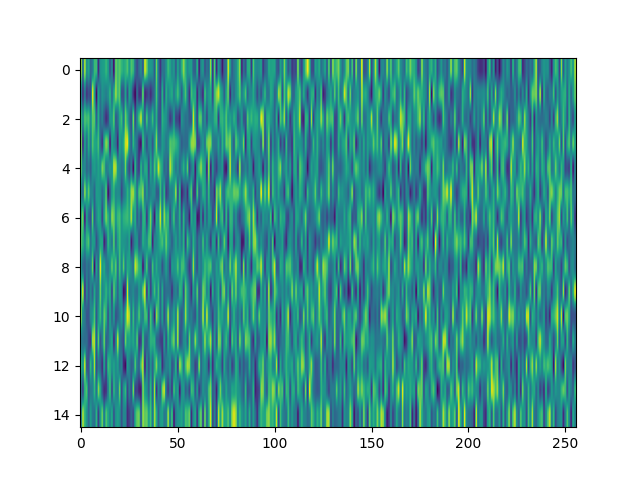
\includegraphics{formality_embedding.png}

It is clear that the learned formality embedding was non-trivial. The difference between the formal and the informal embeddings also appear to be closer for neighbouring positions in the sentence (y-axis), consistent with what our procedural formality classifier does (looking out for the conjugation of the final verb).

We also observe the surprising consistent increase in sentence reconstruction BLEU score. Not only is our decoder able to recover from the additive embedding (a linear shift in the word embedding space), it seems to be able to leverage that information to generate more accurate sentences. It is worth studying whether such a phenomenon can be generalised into other cases with other classes, potentially ones that were generated in unsupervised fashion and/or those that do not have linguistic significance, and leveraged to improve translation quality.

\subsection{Back Translation}

We finally move on to our goal of building a formality-aware translator. The problem with this is, we do not have parellel corpora between two strongly formality-typed languages (such as Japanese and Korean), which would allow us to use our procedural formality tagger to determine the quality of the formality-aware translation by our model. 

In order to get around this problem, we built a formality-aware back-translator. The model consists of two parts that are trained sequentially: a forward-translator and classifier, which takes a strongly formality-typed sentence (in our case, Japanese) and outputs a translation (in English) as well as a formality class; a backward-translator, which takes a sentence in the target language (English) and translates it back to the source language (Japanese). The output of the entire pipeline could then be evaluated for its formality awareness.

For our base Japanese to English translator-classifier, we use the same model architecture as the one we trained for section $3.1$. We were able to achieve $24.4$ BLEU score (compared to $26.3$ for the baseline translator without classifier), while the formality classification accuracy was $.993$, comparable to the one trained alongside Japanese autoencoders. 

We next build a vanilla backward-translator that was trained solely on the translation objective. The baseline back-translator had a BLEU score of $19.1$ and a RIBES score of $27.9$ (pleae refer to section $4$ for details). The back-translated Japanese sentences had a formality awareness of $.269$.

\subsection{Formality-Aware back-translation}

As is the case with the previous section on sentence reconstructors, there are multiple approaches which can all lead to formality-aware back-translation.

\subsubsection{Formality-Aware Back Translation with Joint Training Objectives}

We add the formality awareness joint training objective to the base backward-translator, adding a loss term according to whether the pre-trained encoder-classifier considers the back-translated sentence to have the correct formality. We were able to achieve $18.2$ BLEU score, $29.0$ RIBES score, as well as $.382$ formality reconstruction accuracy (which beat the benchmark of $.269$). As mentioned previously, formality reconstruction accuracy is often upper-bounded by the quality of the translation: a translated sentence that was so malformed that it lacks a formality cue (such as a properly conjugated verb) would obviously fail the formality awareness test. However we note that this is not the case here. We observe the following:

\begin{enumerate}[label=\arabic*]
    \item The model was relatively unconfident about its formality awareness (the pre-trained encoder-classifier gave a formality accuracy of around $60\%$)
    \item While the back-translation quality was poor, the sentences are generally grammatical and contain a properly-conjugated final verb (as assessed by a human on a random sample of $100$ sentences)
\end{enumerate}

We therefore conclude that there is potential for more aggressive formality forcing on the backward-translator, and that formality awareness was not predominantly constrained by translation quality. As such, we decide to apply formality-dependent embeddings on the encoder output, similar to what we did with the sentence reconstructor.

\subsubsection{Back Translation with Multiplicative Formality Embedding}

We next try applying a learned multiplicative formality embedding on the backward encoder output before passing it as argument to the backward decoder, hoping that it would allow us to control the decoder to emit sentences according to their original formality. We were able to get a BLEU score of $14.1$, a RIBES score of $26.6$, and a formality awareness of $.644$: while the base translation quality clear regressed, the formality awareness greatly increased, satisfying our objectives.

We next experiment with different weights for the translation and formality awareness components of the training objective, just as we did with the previous section with sentence reconstructors.


\begin{tabular}{ c c c c }
    Back-translation loss weight & Formality reconstruction accuracy & BLEU score & RIBES score \\
    $.9$ & $0$ & $0$ & $0$ \\
    $.75$ & $.672$ & $13.6$ & $25.6$ \\
    $.5$ & $.644$ & $14.1$ & $26.6$ \\
    $.09$ & $0$ & $0$ & $0$ \\
    $.0099$ & $0$ & $0$ & $0$ \\
\end{tabular}

\subsubsection{Back Translation with Additive Formality Embedding}

Next we experiment with the additive formality embedding scheme, which had yielded superior results for the sentence reconstruction setting. We start of by giving equal weights to back translation loss and formality awareness loss. We measured a BLEU score of $15.8$, a RIBES score of $32.0$, and a formality awareness of $.259$. We observe that while the system's translation quality was relatively unaffected, the formality awareness failed to beat the benchmark of $.382$. We therefore conclude that additive formality embedding is not powerful enough for enforcing formality on the back-translated output.

\section{Evaluation metrics}

We propose a number of different ways to evaluate the translation quality and the sentence reconstruction quality for our different tasks. We analyse the level of correlation between these different metrics on different tasks.

\subsection{Alignment BLEU score}

We use the NLTK toolkit \cite{NLTK} to evaluate the BLEU score of our translations or sentence reconstructions. BLEU score is calculated as the proportion of n-gram overlaps between the hypothesis and the reference; due to only having a single sentence per training data point, such a score is not necessarily a good estimate of the model quality. It also doesn't have a good correlation with sentence formality.

\subsection{Alignment RIBES score}

The NLTK toolkit \cite{NLTK} also supports RIBES score. RIBES evaluates similarly to BLEU, but it is more lenient in terms of the ordering of tokens. This is not to say that RIBES doesn't care about the location of different parts of speech at all; it just doesn't punish it as harshly. This is useful for languages like Japanese, where the purposes of phrases in the sentence are determined by the article/tag characters attached to them rather than through order. As such, we looked at RIBES score as well, and as expected, our RIBES scores were generally about 2 times better than corresponding BLEU scores early into training but only a few points better later on. 

\subsection{Manual, Human Evaluation}
To manually evaluate the translations with human eyes, we randomly sampled 261 (an arbitrary but large enough number) sentences. Among these sentences, we noticed certain patterns in both successful translations and potentially questionable ones. 

The first type of common difficulty was cases where the Japanese sentences omitted some sort of information in the sentence, likely due to it being obvious contextually. Unfortunately for the machine, it is not given this context, so it must sometimes translate incomplete sentences and essentially make an educated guess at certain contexts. Sometimes, it actually manages to do a good job at this, preserving the overall meaning of the phrase. For example: 

"5百万回も見られることになりました"  is translated into: 

"Seen five million times."

In this case, the Japanese sentence is missing a subject. “Seen five million times” is a good word-for-word translation, but any Japanese person would understand that there’s some object that being seen. Without contextual knowledge, the best way to handle this may be to use a generic pronoun, such as “it,” creating the sentence, “it will be seen five million times.” In this sentence specifically, the information contained in “will be” is also missing from our translation. Many other translations of this same structure were also missing tense information though, so we suspect that it has something to do with time-determiners like “will” or “has” being treated as attached to a subject; ie. they would be missing should the subject be missing.

There are some sentences where the translation loses information, though in many of these cases, the translation in still reasonable and sometimes even more reasonable without context. For example:

"何するんだサイラス" is translated into

"What are you doing Cyrus?"

The translation provided in the parallel corpus is, “what the hell are you doing, Cyrus?” The “the hell” part got left out, but there’s no word in the Japanese sentence the means “the hell.” That information would entirely be gained from context or tone. As such, this is an interesting case where context-aside, the machine translation might be considered better than what a BLEU or RIBES score might say. Of course, this still speaks to the machine’s weakness in situations where it does need to know context.

Finally, there are some sentences where the translation adds information. These are rare, and it’s hard to find a pattern in why it’s occurring, as the situations in which it occurs are varied. Often times the additions are conjunctions or articles rather than full on noun or verb phrases. For example: 

"ジョーンズは味方だよ" is translated into

"and jones is on our side."

The translation is pretty accurate, but the “and” is completely new information created by the translator. One could suspect that it has something to do with Katakana being present in the sentences, as Katakana is often used to loan/foreign words that needs to just be sounded out. This happens in cases without Katakana, and the Katakana is those cases is usually translated correctly without showing any other obvious errors stemming from an issue relating to its use, so we think that this is not the case. 

The patterns mentioned are the ones seen most often when the translations are close but not perfect. Aside from these, most incorrect translations just fail to capture the meaning entirely or are absurd. Some are closer than others, of course, but once they’re not close enough to correct, it’s difficult to spot meaningful patterns.

\subsection{Formality Class accuracy}

Our model's understanding of formality is undoubtedly one of the most important aspects of its performance. For the purpose of this study, we evaluate the formality awareness of the sentences generated by the model by passing them through the procedural formality classification system we used to tag our corpus with formality labels.

A limitation to this approach, similar to what happened when we were generating our corpus formality tags, was that there are sentences that do not contain any formality marker: ie. sentence that contain no conjugated verb or adjective, or sentences with "inconclusive" formality. While this is not really an issue during corpus tagging (we removed all inconclusive sentences), this problem is very pronounced when testing on generated sentences, since many are not grammatically well-formed and cannot have their formality measured. As such, there is a level of correlation between translation quality and sentence formality awareness.

All the "formality awareness" results in our study are measured by the ratio of generated sentences that had the correct formality as measured the procedural tagger, over the total number of sentences. The total number of sentences include any inconclusive sentences which may have been generated. 

\subsection{Other evaluation metrics}

Here we briefly discuss other evaluation metrics that we considered using but which didn't make it into the final pipeline.

\subsubsection{Sentence Embedding Similarity}

Comparing the embedding similarity of two sentences is hardly a trivial problem. In order to make our evaluation task tractable, we use a rather trivial construction where we define the embedding of a sentence as the average embedding of all word embeddings in the sentence. We then define sentence similarity as the dot product between the embedding of the two sentences. 

We observe that, while such an approach would allow for the model to learn directly from the final evaluation metric (since the sentence embedding similarity could be back-propagated), it would additional complexity and thus computation overhead to our existing pipeline due to the need for a sentence embedder. It is also not immediately obvious whether a pre-trained sentence embedding should be used, or whether we should train a separate encoder instead. Finally, sentence embedding similarity has no obvious connection to our ultimate goal: formality-aware translation. As such, we decided against using sentence embedding similarity as our evaluation metric.

\section{Future work}

\subsection{Potential improvements to procedural formality evaluation}

In section $2$ we introduced our procedural formality evaluation, which is grounded in the morphology of the languages that we studied and quite accurate empirically. However, this evaluation method is also discrete and non-differentiable, meaning that it could not be used as the training objective for a neural model. The encoder-classifier setup that we used as the neural formality classification objective does not correlate with our procedural formality classifier well. 

This is one aspect where earlier studies that relied on n-gram counting for formality classification would have an advantage. By applying an F-measure on formality-specific n-gram overlap, we can have a back-propagable metric that correlates with linguistic formality.

\subsection{Can formality encoding be transferred?}

A non-trivial question arising from our studies is the potential to perform domain adaptation/transfer of our model. Given the simplicity of our classifier, for the classification result from our language-dependent encoders to be transferrable across languages, we would necessarily need to align our word embeddings across different languages for a continual learning/transfer learning task to succeed. This is an area that merits further study.

\subsection{Can our work be generalised to other multi-domain scenarios?}

At a high level, our model can be thought of as explicitly applying a context (a manually extracted hidden state) onto the encoder output, prior to word emission with our decoder. In our case, the context is a representation of the formality of the input sentence.

A number of other types of context could be used to improve translation quality. They could reflect some kind of domain information (emission language, emotion, politeness, etc.). They could also used as a contextual memory, helping the decoder to emit phrases or words that are more appropriate given the recent semantic context or the document context.

\newpage
\printbibliography
\end{document}
